\documentclass[conference]{IEEEtran}
\usepackage{blindtext, graphicx}
\usepackage{cite} 
\usepackage{csquotes}
\usepackage[hidelinks]{hyperref}
\usepackage{url}

\hyphenation{op-tical net-works semi-conduc-tor}

\begin{document}
\title{MCAST IICT Research Paper}

% The sequence of authors in a paper has meaning. The first to be listed is known as the First Author, who is usually the student and/or the person doing the bulk of the work. The next in line, provided that there are two persons, is called the corresponding author, also known as the technical mentor/supervisor. Any person who is consulting, correcting or verifying such as a second reader or senior person within the Faculty/Institute is listed after the previous authors.

\author{\IEEEauthorblockN{Joe Borg, Lisa Abela, ICTAR Group}
\IEEEauthorblockA{Institute of Information \& Communication Technology\\
Malta College or Arts, Science \& Technology\\
Corradino Hill\\
Paola PLA 9032\\
\{joe.borg, lisa.abela, ictar\}@mcast.edu.mt}}

\maketitle

\begin{abstract}
This paper offers some additional guidelines for MCAST IICT 2nd year B.Sc. students on research paper writing. The abstract is the first paragraph that any researcher reads and thus you need to capture the essence of your research. Dedicate 1 sentence for the theme (subject matter), another for your project aim, one for the proposed solution, then for the general outcome of this project (positive/negative result/outcome), another for the technology used (Windows/Linux, Android/iOS, C\#/Java, Unity/Unreal), finally for any technique used (Neural Networks, Pearl Noise, Market Basket Analysis, K-Means, HMM, Augmented Reality). Following is an example: \textit{In this research we are tackling the automatic annotation of cast members and use of key props within movies. Movies tend to gather a huge fan gathering who dedicate a lot of time and resources for documenting the content, thus tools to automate processes such as the timeline when cast members appear, presents of props such as weapons and other forms of annotations are desired. In this research we propose the use of image processing techniques, namely Principal Component Analysis (PCA) and Convolutional Neural Networks (CNN) for the automatic annotation of actors' timeline and presence of weapons in the popular Tv series Game of Thrones (GoT). Our proposed solution managed to detect the targets in 85\% of the cases and we identify situations where this is challenging and recommend future research directions.}
\end{abstract}

\begin{IEEEkeywords}
%3 to 5 words/phrases about the key aspects of your research, theme, technology, technique
MCAST, IICT, \LaTeX, Project, Paper
\end{IEEEkeywords}

\IEEEpeerreviewmaketitle

\section{Introduction}
\label{sec:Int}
\par The introduction is intended to give a more detailed overview of the research from the abstract. Document the \textbf{theme}, the \textbf{aim} and \textbf{motivation}. By motivation we mean the justification to why this project/research is relevant/needed for the current year/period and for your specific area of studies. You can consider also including your \textbf{hypothesis} and \textbf{research questions} in this section. Conclude this section with an overview of what to expect in the next sections. It is good practice to cross-reference your own paper using the ref command for the matching section label, such as in Section~\ref{sec:Lit} a review of current research is found.
\section{Literature Review}
\label{sec:Lit}
\par Give a \textbf{brief} overview of the theme, history and facts. You should use the present tense since what you are documenting is current knowledge. Do not dedicate a lot to historical facts about the subject matter, but limit to a paragraph. Make sure you quantify by quoting statistics where relevant. Following is an example for a research in \enquote{Automatic cyber-bullying detection}: \textit{With the popularity of social media, predominantly amongst the adolescent and young adult generations, there appears to be a correlation between the increase in suicide rates and social networking adoption~\cite{miron2019suicide}, with suicide attempts increasing by 10\% amongst adolescents and by 5.6\% amongst young adults for the period 2013-2017.} 

\par Once you have documented some background on the theme you need to focus on three key aspects: \textbf{Data set}; \textbf{Algorithms}; \textbf{Evaluation}. So you need to research existing data sets and document them. Say we want to explore accent recognition in audio/video clips, you would need to identify existing data sets and document first by enumerating then by comparing in a table layout such as in Table~\ref{tab:Data}. A useful tool for creation of tables is Truben's Table Tool\footnote{\url{http://truben.no/table/}}. When enlisting the data sets make sure you provide the proper citation. When comparing you need to identify the key features/factors/variable that are important for your subject matter.

\begin{enumerate}
    \item The Accents of the British Isles (ABI-1) Speech Corpus, \cite{d2004accents}
    \item TIMIT Acoustic-Phonetic Continuous Speech Corpus, \cite{garofalo1993darpa}
    \item Common Voice Data Set, \cite{common_voice}
    \item WSJCAM0 Corpus, \cite{robinson1995wsjcamo}
    \item The Speech Accent Archive, \cite{weinberger2011speech}
    \item The Arctic CMU Audio Database, \cite{kominek2004cmu}
    \item VoxCeleb2, \cite{chung2018voxceleb2} 
\end{enumerate}

\begin{table}[ht]
    \caption{Data-set comparison. Accent: Native (N); Non-Native (NN)}
    \label{tab:Data}
    \centering
    \begin{tabular}{l|l|l|l|l|l}
        \textbf{Data set} & \textbf{Speakers} & \textbf{Utterances} & \textbf{Accents}   & \textbf{Citations} & \textbf{Type} \\\hline
        1               & 280               & 855                 & 14                & 28              & N               \\
        2               & 630               & 6,300               & 8                 & 1,918           & N               \\
        3               & 50,590            & 644,120             & 16                & N/A             & N \& NN            \\
        4 & 140 & 4,400 & 4 & 346 & N \\
        5               & 2,140             & 2,140               & \textgreater{100} & 132             & N \& NN        \\
        6               & 18                & 1,150               & 4                 & 458             & N \& NN               \\
        7               & 6,000              & 1,128,246          & 6                 & 168             & N \& NN  
    \end{tabular}
\end{table}

\par Next you need to provide an overview of what researchers have proposed and their key results. A survey or review paper would be ideal since these kind of papers would cover multiple techniques and provide good comparisons. Returning to our example of \enquote{Automatic cyber-bullying detection} consider the technique comparison documented in Table~\ref{tab:Com}. Note the structure used in this table, first you have the citation of the research, followed by the data set used, then the metric quoted for comparison, finally the relevant result. 

\begin{table}[ht]
    \centering
    \caption{State of the art results}
    \label{tab:Com}
    \resizebox{\columnwidth}{!}{
        \begin{tabular}{l|l|l|l}
            \textbf{\textbf{Study}}         & \textbf{\textbf{Data set}}    & \textbf{\textbf{Metrics}} & \textbf{\textbf{Results}}                                                                   \\ \hline
            \cite{prathyusha2017cyberbully} & Crime Investigation Forum    & F1 Score                  & \begin{tabular}[c]{@{}l@{}}CDMS: 40.75\%\\ CDCSGF: 39.75\%\end{tabular}                     \\ \hline
            \cite{van2018automatic}         & Corpus for English and Dutch & F1 Score                  & \begin{tabular}[c]{@{}l@{}}English: 64\%\\ Dutch: 61\%\end{tabular}                         \\ \hline
            \cite{al2016cybercrime}         & Twitter                      & F1 Score                  & 93.6\%                                                                                      \\ \hline
            \cite{zhong2016content}         & Instagram                    & F1 Score                  & \begin{tabular}[c]{@{}l@{}}SVM Classifier: 95.00\%\\ Image Classifier: 68.08\%\end{tabular} \\ \hline
            \cite{reynolds2011using}        & Formsrping                   & Accuracy                  & 78.5\%                                                                                      \\ \hline
            \cite{dinakar2011modeling}      & Youtube                      & Accuracy                  & 66.70\%        \\   \hline        
        \end{tabular}
    }
\end{table}

\par The final recommended part in a good literature review is a review in the evaluation metrics used. It is not possible to cover all possible evaluation metrics but in most cases there is a classification problem, which would require something called a confusion matrix. Consider the problem of recognising and distinguishing an image of a cat from that of a dog. You will have a data set split into training and testing. Both will have the ground truth, what the image is actually showing. This ground truth, in the case of the training data set will be used for the creation of the Artificial Intelligence (AI) model, whilst the ground truth in the testing data set will be used to compare the predicted classification. The predictions are plotted in a confusion matrix as shown in Table~\ref{tab:CatDog}. The same table can be extended to have more than 2 categories such as introducing the mouse category. Then you need to cycle the focus for each category as shown in Table~\ref{tab:CatObjective} and Table~\ref{tab:DogObjective}, then extract the key values namely:
\begin{enumerate}
    \item \textbf{True Positives (TP)} - This refers to the correctly predicted positive values i.e. the value of both the actual class and predicted class is yes. 
    \item \textbf{True Negatives (TN)} - These are the correctly predicted negative values i.e. the value of both actual class and predicted class is no.
    \item \textbf{False Positives (FP)} - It indicates values where the actual class is no but the predicted class is yes.
    \item \textbf{False Negatives (FN)} - It indicates values where the actual class is yes but the predicted class in no.
\end{enumerate}

\begin{table}
    \caption{Sample Cat vs Dog Confusion Matrix}
    \label{tab:CatDog}
    \centering
    \begin{tabular}{ll|ll}
    ~      & ~   & \textbf{Predicted} & ~   \\
    ~      & ~   & Cat       & Dog \\ \hline
    \textbf{Actual} & Cat & 33        & 2   \\
    ~      & Dog & 5         & 30  \\
    \end{tabular}
\end{table}

\begin{table}
    \caption{Cat category evaluation metrics}
    \label{tab:CatObjective}
    \centering
    \begin{tabular}{ll|ll}
    ~      & ~   & \textbf{Predicted} & ~   \\
    ~      & ~   & Cat       & Not-Cat \\ \hline
    \textbf{Actual} & Cat & TP        & FN   \\
    ~      & Not-Cat & FP         & TN  \\
    \end{tabular}
\end{table}

\begin{table}
    \caption{Dog category evaluation metrics}
    \label{tab:DogObjective}
    \centering
    \begin{tabular}{ll|ll}
    ~      & ~   & \textbf{Predicted} & ~   \\
    ~      & ~   & Not-Dog       & Dog \\ \hline
    \textbf{Actual} & Not-Dog & TN        & FP   \\
    ~      & Dog & FN         & TP  \\
    \end{tabular}
\end{table}

\par The confusion matrices are used to provide evaluation metrics such as Accuracy, Precision, Recall and F1-Score. Depending on the subject matter being researched the proper metrics need to be quoted, thus the need to research this in academic literature. For a quick but reliable reference you can consider Wikipedia's dedicated page\footnote{\url{https://en.wikipedia.org/wiki/Confusion_matrix}}.

\begin{enumerate}
    \item \textbf{Accuracy (ACC)} - This shows the measure of effectiveness of the machine learning model.
    \begin{equation} 
     Accuracy (ACC)= \frac{TP + TN}{P + N}
    \end{equation}
    \item \textbf{Precision (PPV)} - Precision is the ratio of correctly predicted positive values to the total predicted positive values. This metric highlights the correct positive predictions out of all the positive predictions. High precision indicates low false positive rate.
    \begin{equation} 
     Precision (PPV)= \frac{TP}{TP + FP}
    \end{equation}
    \item \textbf{Recall (TPR)} - The recall is the ratio of correctly predicted positive values to the actual postive values. Recall highlights the sensitivity of the algorithm i.e. out of all the actual positives how many were caught by the program.
    \begin{equation} 
     Recall (TPR)= \frac{TP}{P}
    \end{equation}
    
    \item \textbf{F1 Score} - F1 Score is the weighted average of Precision and Recall. Therefore, this score takes both false positives and false negatives into account. Intuitively it is not as easy to understand as accuracy, but F1 is usually more useful than accuracy, especially if you have an uneven class distribution.
    \begin{equation} 
     F1 Score = \frac{2TP}{2TP + FP + FN}
    \end{equation}
\end{enumerate}

\section{Research Methodology}
\label{sec:Res}
\par This section is one of the most important parts of your research and it is the one that will receive most criticism. The reason is that here you document how you conducted your research. Since you are reading a B.Sc. degree you are expected to follow a scientific method, thus in this section you are expected to document: \textbf{the problem}; \textbf{hypothesis}; \textbf{aim \& objectives}; \textbf{research questions}; and \textbf{research pipeline}. Let's go through each.

\par First start by providing a brief overview of the problem, similar to what you already mentioned in the previous sections. Then provide a hypothesis, this is the assumption you are making, which via your research you are attempting to prove or disprove. An example hypothesis in traffic management would be: \textit{By using image processing on public camera video feeds we believe that it is possible to estimate the traffic congestion at a higher precision than public traffic data feeds.}

\par After explaining the problem and hypothesis you need to specify why you are doing this research and what you think the output will be, so the aim \& objectives. Let us consider the \enquote{Marine Vessel Tracking} concept: \textit{With this research we aim to be able to automatically detect any anomalies within Marine traffic, such as drug smuggling, human trafficking and/or collisions.} Our objectives are:
\begin{enumerate}
    \item Identify existing data sets and manners of connecting them or even enriching them.
    \item Review existing algorithms and propose a suitable model
    \item Evaluate the effectiveness of the proposed model with real data and existing research.
\end{enumerate}

\par So lastly you have to present a number of research questions that you attempt to answer, which ideally revolve around the \textbf{data set}, \textbf{algorithm} and \textbf{evaluation} which you documented in your literature review:
\begin{enumerate}
    \item Does a data set need to be created for such a research?
    \item Which current technology is best suited to address the problem?
    \item How does the proposed solution compare with existing solutions?
\end{enumerate}

\par Finally, you need a plan on how you intend to answer the research questions which will help you prove/disprove the hypothesis. Different research areas would require specific pipelines, yet a generic one is shown in Fig~\ref{fig:Pipeline}. After presenting an illustration of your pipeline it is recommended to documenting what has been done at every stage. Remember you should use past tense in this section since you are document what you have already done, since this paper will be published at the end of your research.

\begin{figure}[ht]
    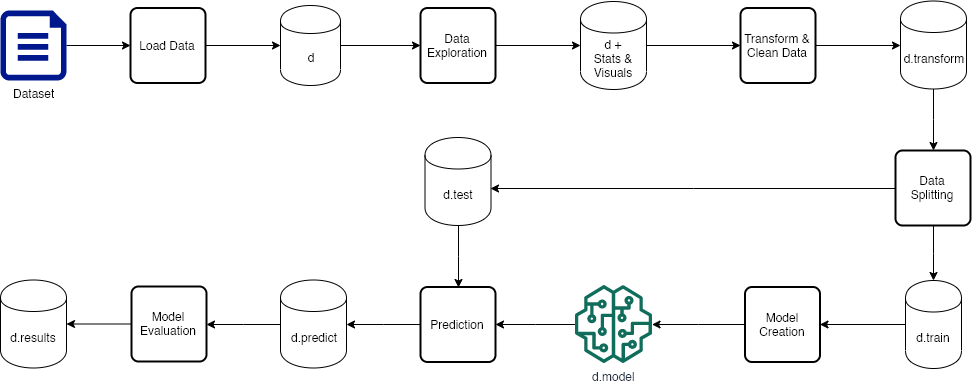
\includegraphics[scale=0.25]{includes/pipeline.png}
    \centering
    \caption{Research Pipeline}
    \label{fig:Pipeline}
\end{figure}
\section{Findings \& Discussion of Results}
\label{sec:Fin}
\par This section is a delicate section and you are encouraged to be as honest and open as possible. The aim is not to show that you got a perfect solution to a long existing problem. Trying to state that in a few months you developed a perfect solution with 100\% is not convincing and raises doubts. It is recommended that you document your findings in every step of your research pipeline, highlighting your observations and decisions taken. Present your results and very importantly compare with existing research which you documented in Section~\ref{sec:Lit}. 

\par The focus of the Project module is for you to delve into an area that exposes you to new technologies and offers you an opportunity to be critical of your work. So you are expected to document where your solution/research worked and where it did not. Reflect and document reasons why the solution/research did not perform as expected and propose ways of addressing this. From these observations you will produce new research questions in the next section. Consider the research in \enquote{Brand usage detection within audio streams}, where certain key terms were searched within videos, the results of which are documented in Table~\ref{tab:Accents}. You will notice that the terms \enquote{Peppa} and \enquote{Sushi} were the least recognised terms even by the best transcribers. Upon investigation we determined that \enquote{Peppa} was not recognised cause of voice morphing to create childish voices in the cartoon video, whilst \enquote{Sushi} was pronounced by a Japanese person speaking English. So the research student decided to focus his dissertation research on how to create a system that is able to recognise heavy accents to automate the configuration of a transcriber, in this case to cater for English spoken by a Japanese person, which accent is very different from an Indian accent, British accent or Italian accent, just to name a few.

\begin{table}[ht]
    \centering
    \caption{Recall results}
    \label{tab:Accents}
    \begin{tabular}{l|l|l|l|l}
    \textbf{\#} & \textbf{Term}   & \textbf{Google} \textbf{Cloud} &\textbf{} \textbf{Google} \textbf{Speech} & \textbf{Sphinx} \textbf{CMU} \\ \hline
    1        & Peppa  & 27\%             & 33\%              & 0\%        \\
    2        & Peppa  & 33\%             & 22\%              & 0\%        \\
    3        & Apple  & 96\%             & 92\%              & 79\%       \\
    4        & Galaxy & 100\%            & 100\%             & 100\%      \\
    5        & Galaxy & 95\%             & 95\%              & 80\%       \\
    6        & Sushi  & 75\%             & 35\%              & 0\%        \\ \hline
    ~       & Average & 71\%    & 62\%  &   43\%    \\
    \end{tabular}
\end{table}
\section{Conclusion}
\label{sec:Con}
So the conclusion is most probably the second section that a reader would use to consider reading in full your research. Thus it is important to highlight the essence of your research. The recommended approach is to answer your research methodology. Start by answering your research questions, then stating to what degree did this research achieve its aim and objectives, highlighting potential causes for not being able to do so at a desired level, such as time, or other circumstances. Consider the following: \textit{A student was due to research the use of MCAST computers during out-of-office hours to offer a private cloud computing service for research, similar to Google Cloud but free for MCAST students. Due to the lock-down by COVID-19 pandemic we could not continue on the original planned research objective and had to adapt.}
\par The final and most important part of the conclusion are your recommendations for future research, not necessarily for yourself (referring to what you plan to do in your dissertation or beyond), but also to other future researchers who might consider doing similar work to yours. The recommendations you provide here will set such prospective researchers on a better track/direction thanks to your experience.

\appendices
\section{Supporting material}
You can add screen shots and statistics. Stick to essential information.
\section*{Acknowledgement}

You can dedicate this section for special assistance that you were given by a 3rd party. Not your mentor, relatives or questionnaire participants.

\bibliographystyle{IEEEtran}
\bibliography{sources.bib}

\end{document}


